\documentclass{scrartcl}

\usepackage[utf8]{inputenc}


% zus�tzliche mathematische Symbole, AMS=American Mathematical Society 
\usepackage{amssymb}
\usepackage{amsmath}
\usepackage{amsthm}
\usepackage{bbm}
\usepackage{color}
\usepackage{listings}
\usepackage{pdfpages}
\usepackage{csquotes}

% f�rs Einbinden von Graphiken
\usepackage{graphicx}

% f�r Namen etc. in Kopf- oder Fu�zeile
\usepackage{fancyhdr}
\usepackage{tikz}
\usetikzlibrary{arrows, automata}

% erlaubt benutzerdefinierte Kopfzeilen 
\pagestyle{fancy}

% Definition der Kopfzeile
\lhead{
\begin{tabular}{lll}
Johannes Kalmbach &  &   \\
\end{tabular}
}
\chead{}
\rhead{\today{}}
\lfoot{}
\cfoot{Seite \thepage}
\rfoot{} 

\begin{document}

\section*{Deep Learning Lab, Report for Submission 2}

\subsection*{Exercise 4, Random Search}
The best configuration that was found during my experiments with the given settings was:
\begin{itemize}
	\item learning rate: $0.08847$
	\item batch size: 46
	\item filter size: 3x3
	\item number of filters per layer: 63
\end{itemize}
After training this setup for the full 12 epochs it achieved an error rate on the test set of \textbf{0.98\%} which is much better than what I could achieve with the feed forward networks from two weeks ago. \\
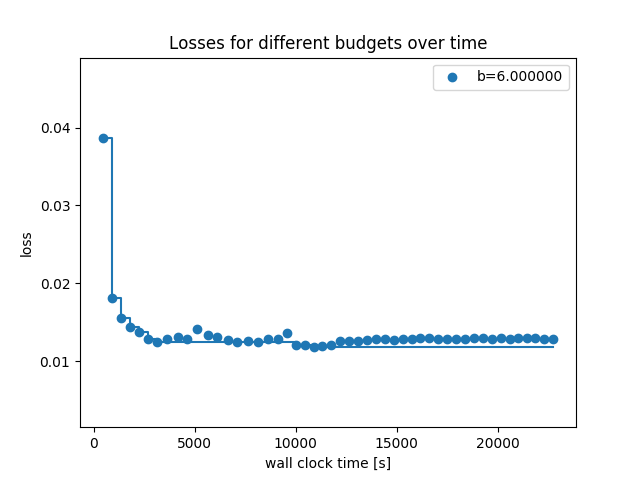
\includegraphics[scale=0.7]{random_result.png}

\end{document}


